\chapter{线性代数}
\label{chap:linear_algebra}
\section{矩阵和向量}

矩阵是从许多实际问题中抽象得来的数学概念,是整个线性代数学科的基础,
在自然科学,工程数学和国民经济中有着广泛的应用。在机器学习领域,
大部分计算方法都是以矩阵的形式进行,因此学习矩阵的性质和计算显得尤为重要。

矩阵的定义是$m*n$个数$a_{ij}$($i=1,2,\cdots,m;j=1,2,\cdots,n$)排成$m$行$n$列的矩阵数表。
这样的一个数表称为$m*n$矩阵,简称为矩阵,$a_{ij}$也被称为矩阵的第$i$行第$j$列元素。

\begin{equation}
	\left( \begin{matrix}
    a_{11} & a_{12} & \cdots & a_{1n}\\
    a_{21} & a_{22} & \cdots & a_{2n}\\
    \vdots & \vdots & \ddots & \vdots\\
    a_{m1} & a_{m2} & \cdots & a_{mn}
\end{matrix}
\right )
\end{equation}

特殊的,当m=1时,矩阵$A=(a_{1},a_{2},\cdots,a_{n})$被称为行矩阵,也叫$n$维行向量;
同样的,当n=1时,矩阵$A=\left( \begin{array}{ccc}{b_1} \\{b_2}\\\vdots\\{b_m}\end{array}\right)$
被称为列矩阵,也称为$m$维列向量;当m=n时,矩阵$A=(a_{ij})_{n*n}$称为$n$阶矩阵或$n$阶方阵,
也可记为$A_{n*n}$。

\begin{figure}
	\centering
	\tikzstyle{arrow} = [thick, ->, >= stealth,red]
	\begin{minipage}[c]{0.5\textwidth}
	\centering
		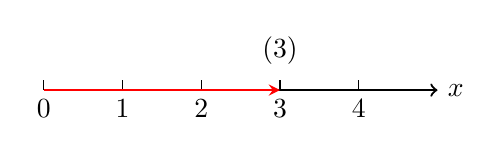
\begin{tikzpicture}
			\pgfmathsetmacro{\ticker}{0.125}
			 \draw [->,thick] (0,0) node (yaxis) [above] {}
							|- (5,0) node (xaxis) [right] {$x$};
			 \foreach \i/\texti  in {0,1,2,3,4} {
			 \draw (1*\i,0) --(1*\i,\ticker) node[label=below:\texti]{};
			 }
			 \draw[arrow] (0,0)--(3,0);
			 \node at (3,0.5) {$(3)$};
			\end{tikzpicture}
			\caption{一维向量示意图}
			\label{one_dimension_vector}
	\end{minipage}%
	\begin{minipage}[c]{0.5\textwidth}
	\centering
	 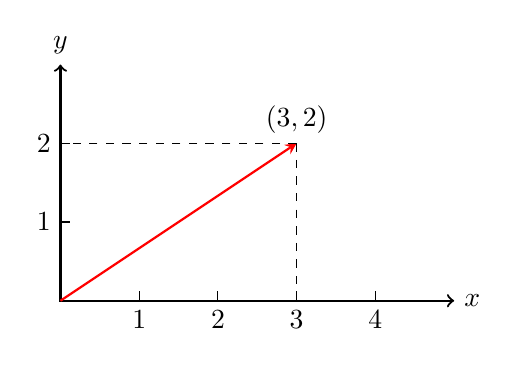
\begin{tikzpicture}
			\pgfmathsetmacro{\ticker}{0.125}
			\draw [<->,thick] (0,3) node (yaxis) [above] {$y$}
							|- (5,0) node (xaxis) [right] {$x$};
			\foreach \i/\texti  in {1,2,3,4} {
			\draw (1*\i,0) --(1*\i,\ticker) node[label=below:\texti]{};
			}
			\foreach \j/\textj  in {1,2} {
			\draw (0,1*\j) --(\ticker,1*\j) node[label=left:\textj]{};
			}
			\draw[arrow] (0,0)--(3,2);
			\draw[dashed] (3,2)--(3,0);
			\draw[dashed] (3,2)--(0,2);
			\node at (3,2.3) {$(3,2)$};
			\end{tikzpicture}
			\caption{二维向量示意图}
			\label{two_dimension_vector}
	\end{minipage}
	\end{figure}

向量指的是既包含大小,又包含方向的一类量,例如位移,速度,加速度,力等,又称为矢量。
在线性代数中,向量可以用矩阵的形式进行表示,例如一个一维的向量可以用向量$A=\left( \begin{array}{ccc}{a_{1}}\end{array}\right)$
表示,二维向量可以用$A=\left( \begin{array}{ccc}{a_{1},a_{2}}\end{array}\right)$表示,如图\ref{one_dimension_vector}和图\ref{two_dimension_vector}所示。
同理,我们可以推出,包含$n$个分量的向量可以称为$n$维向量,用
$A=\left( \begin{array}{ccc}{a_{1},a_{2},a_{3},\cdots,a_{n}}\end{array}\right)$表示。

\begin{figure}[!b]
	\begin{lstlisting}[language=Java]
		public static INDArray create(double[] data, long[] shape) {
	
			checkShapeValues(data.length, shape);
	
			INDArray ret = INSTANCE.create(data, shape, Nd4j.getStrides(shape, Nd4j.order()), DataType.DOUBLE, Nd4j.getMemoryManager().getCurrentWorkspace());
			return ret;
		}
	\end{lstlisting}
	\caption{NDArray的创建}
	\label{NDArray_creation}
\end{figure}

在DL4J中,普通矩阵的创建用create方法实现,源码如图\ref{NDArray_creation}所示。首先我们需要传入两个数组data和shape,
作为源数据组并决定矩阵的形状与维度。然后,系统会调用checkShapeValues方法
来确保输入data数组的长度与shape数组相符。最后,利用这些数据创建一个INDArray并返回,
这就完成了矩阵的创建。

特殊的,我们可以用简便的方法来创建部分简单的矩阵,例如zeros()方法可以创建一个全零矩阵,
仅需要传入行数和列数即可。同理还有ones(),valueArrayof()等方法。


\subsection{基本运算}

\begin{figure}[!ht]
	\centering
	\begin{minipage}[c]{0.5\textwidth}
	\centering
		\begin{equation*}
	    \left( \begin{matrix}
        a_{11} & a_{12} & \cdots & a_{1n}\\
        a_{21} & a_{22} & \cdots & a_{2n}\\
        \vdots & \vdots & \ddots & \vdots\\
        a_{m1} & a_{m2} & \cdots & a_{mn}
        \end{matrix}
        \right )
		\end{equation*}
		\caption{矩阵$A$}
		\label{matrix_a}
	\end{minipage}%
	\begin{minipage}[c]{0.5\textwidth}
	\centering
    \begin{equation*}
	    \left( \begin{matrix}
        b_{11} & b_{12} & \cdots & b_{1n}\\
        b_{21} & b_{22} & \cdots & b_{2n}\\
        \vdots & \vdots & \ddots & \vdots\\
        b_{m1} & b_{m2} & \cdots & b_{mn}
        \end{matrix}
        \right )
		\end{equation*}
		\caption{矩阵$B$}
		\label{matrix_b}
	\end{minipage}
\end{figure}

矩阵有四种运算:加减、数乘、乘法和转置。下面我们将用例子展示矩阵的运算,
假设我们有两个矩阵$A$和$B$,如图\ref{matrix_a}与图\ref{matrix_b}所示。

\subsubsection{矩阵的加减}

$A$和$B$是两个$m*n$型矩阵,那么存在矩阵$C$,记$C=A+B$,称$C$为矩阵$A$和$B$的加法运算。
需要注意的是,进行加法运算的两个矩阵行数和列数必须相等,否则无法进行运算。

\begin{figure}[!hb]
			\begin{equation*}
				\left( \begin{matrix}
					a_{11}+b_{11} & a_{12}+b_{12} & \cdots & a_{1n}+b_{1n}\\
					a_{21}+b_{21} & a_{22}+b_{22} & \cdots & a_{2n}+b_{2n}\\
					\vdots & \vdots & \ddots & \vdots\\
					a_{m1}+b_{m1} & a_{m2}+b_{m2} & \cdots & a_{mn}+b_{mn}
					\end{matrix}
					\right )
					\end{equation*}
			\caption{矩阵$C$}
\end{figure}

矩阵的加法在DL4J中由add方法和addi方法实现。代码会先检测输入的数组是否为数字矩阵,以此判断
是否可进行加法操作,最后将两个矩阵进行加法操作。


\begin{figure}[!hb]
	\begin{lstlisting}[language=Java]
		public INDArray add(INDArray other) {
	       validateNumericalArray("add", false);
		   return addi(other, Nd4j.createUninitialized(Shape.pickPairwiseDataType
		   (this.dataType(), other.dataType()), this.shape(), this.ordering()));}
	\end{lstlisting}
\end{figure}

\subsubsection{矩阵的数乘}

矩阵$A$是一个$m*n$型矩阵,$k$是一个数,则称矩阵$D$为矩阵$A$与数$k$的乘积,称为数乘,记为$kA$。

\begin{figure}[!h]
	\begin{equation}
		(ka_{ij})_{m*n}=
		\left( \begin{matrix}
			ka_{11} & ka_{12} & \cdots & ka_{1n}\\
			ka_{21} & ka_{22} & \cdots & ka_{2n}\\
			\vdots & \vdots & \ddots & \vdots\\
			ka_{m1} & ka_{m2} & \cdots & ka_{mn}
			\end{matrix}
			\right )
	\end{equation}
	\caption{矩阵$D$}
\end{figure}

矩阵的数乘与加法基本一致,都是先检验是否为数字矩阵的操作,随后对矩阵中的每个元素进行乘法操作。


\begin{figure}[!ht]
	\begin{lstlisting}[language=Java]
	  public INDArray mul(Number n) {
	     validateNumericalArray("mul", false);
		 return muli(n, Nd4j.createUninitialized(Shape.pickPairwiseDataType
		 (this.dataType(), n), this.shape(), this.ordering()));}
	\end{lstlisting}
	\end{figure}

矩阵的加法和数乘运算统称为矩阵的线性运算。矩阵的线性运算满足交换律,分配律和结合律。

\subsubsection{矩阵的乘法}

设$A=(a_{ik})_{m*s}$,$B=(b_{kj})_{s*n}$,定义$A$与$B$的乘积$AB$是一个$m*n$
矩阵$C=(C_{ij})_{m*n}$,$C$的第i行第j列元素等于$A$的第i行元素与$B$的第j列对应元素
乘积的代数和,如图\ref{matrix_e}:

\begin{figure}[!ht]
	\begin{equation*}
		AB=
		\left( \begin{matrix}
			a_{1}b_{1} & a_{1}b_{2} & \cdots & a_{1}b_{n}\\
			a_{2}b_{1} & a_{2}b_{2} & \cdots & a_{2}b_{n}\\
			\vdots & \vdots & \ddots & \vdots\\
			a_{n}b_{1} & a_{n}b_{2} & \cdots & a_{n}b_{n}
			\end{matrix}
			\right )
	\end{equation*}
	\caption{矩阵$E$}
	\label{matrix_e}
\end{figure}

DL4J中,矩阵乘法的源码先对进行乘法操作的两个矩阵判断是否为同一数据类型,之后再得出乘法计算后矩阵的
维度和形状,最后计算后将结果写入结果矩阵,返回结果,如图\ref{matrix_multiply_code}。


\begin{figure}[!ht]
	\begin{lstlisting}[language=Java]
		public INDArray mmul(INDArray other) {
			Preconditions.checkState(this.dataType() == other.dataType(), "Matrix multiplication: 
			    arrays must have same dtype: %s vs. %s", this.dataType(), other.dataType());
			long[] shape = {rows(), other.rank() == 1 ? 1 : other.columns()};
			INDArray result = createUninitialized(this.dataType(), shape, 'f');
			if (result.isScalar())
				return Nd4j.scalar(Nd4j.getBlasWrapper().dot(this, other)).reshape(1, 1);
			return mmuli(other, result);
		}
	\end{lstlisting}
	\caption{矩阵乘法源码}
	\label{matrix_multiply_code}
	\end{figure}


\subsubsection{矩阵的转置}

设存在$m*n$矩阵$A$,则称$n*m$矩阵$B$为$A$的转置矩阵,记为$A^T$。

\begin{figure}[!hb]
	\centering
	\begin{minipage}[c]{0.5\textwidth}
	\centering
		\begin{equation}
	    \left( \begin{matrix}
        a_{11} & a_{12} & \cdots & a_{1n}\\
        a_{21} & a_{22} & \cdots & a_{2n}\\
        \vdots & \vdots & \ddots & \vdots\\
        a_{m1} & a_{m2} & \cdots & a_{mn}
        \end{matrix}
        \right )
        \end{equation}
		\caption{矩阵$A$}
	\end{minipage}%
	\begin{minipage}[c]{0.5\textwidth}
	\centering
    \begin{equation}
	    \left( \begin{matrix}
        a_{11} & a_{21} & \cdots & a_{m1}\\
        a_{12} & a_{22} & \cdots & a_{m2}\\
        \vdots & \vdots & \ddots & \vdots\\
        a_{1n} & a_{2n} & \cdots & a_{mn}
        \end{matrix}
        \right )
        \end{equation}
		\caption{矩阵$B$}
	\end{minipage}
\end{figure}

在DL4J中,矩阵的转置调用了permute方法,先将原矩阵的形状,源数据,排列规则等属性提出并进行转置,
再利用新属性生成一个新的INDArray并返回,在实际使用中我们需要调用transpose()方法即可
完成矩阵的转置。

\begin{figure}[!ht]
	\begin{lstlisting}[language=Java]
		public INDArray permute(int... rearrange) {
	
	       checkArrangeArray(rearrange);
	       int[] newShape = doPermuteSwap(shapeOf(), rearrange);
	       int[] newStride = doPermuteSwap(strideOf(), rearrange);

	       char newOrder = Shape.getOrder(newShape, newStride, 1);

	       INDArray value = create(data(), newShape, newStride, offset(), newOrder);
				 return value;
		}
	\end{lstlisting}
\end{figure}

\subsection{多维空间}

多维空间一般指多维向量空间。一般来说,我们将实数域上的全体$n$维向量构成的集合称为$n$维向量
空间$R^n$。

在此基础上,我们设$\alpha_{1},\alpha_{2},\alpha_{3}...,\alpha_{r}$是向量空间中$V$
中的向量,若它们满足:(1)$\alpha_{1},\alpha_{2},\alpha_{3}...,\alpha_{r}$线性无关;
(2)$V$中的任何一个向量都可以用$\alpha_{1},\alpha_{2},\alpha_{3}...,\alpha_{r}$线性
表示,则称$\alpha_{1},\alpha_{2},\alpha_{3}...,\alpha_{r}$为向量空间$V$的一个基,
$r$称为向量空间$V$的维数,并称$V$为$r$维向量空间。

显然,向量空间的基不是唯一的。同时,我们应该注意到向量的维数和向量空间的维数并不是同一个概念。




\subsection{特征值与特征向量}

设$A$是一个$n$阶矩阵,如果存在数$\lambda$和非零列向量$\alpha$,使得$A\alpha=\lambda\alpha$,
则称$\lambda$为矩阵$A$的一个特征值,称$\alpha$为$A$属于特征值$\lambda$的一个特征向量。

\vspace{5pt}

\begin{figure}[!ht]
	\begin{lstlisting}[language=Java]
		private static void getEigenValue(int[] A){
			int a = 1;
			int b = -(A[0] + A[3]);
			int c = A[0]* A[3] - A[1] * A[2];
			double t = b*b - 4 * (a * c);
			if (t >= 0) {
				double lambda1 = (Math.sqrt(t) - b) * 1.0 / (2 * a);
				double lambda2 = (-(Math.sqrt(t))-b) * 1.0 / (2 * a);
				int[] resultArray1 = {1,(int)((A[2])/(lambda1 - A[3]))};
				System.out.print("矩阵的第一个特征值为" + lambda1 + ",特征向量为" + "[" + resultArray1[0] 
				+ "," + resultArray1[1] + "]");
			}
	  }
	\end{lstlisting}
\end{figure}

代码块展示了简单的二维矩阵计算特征值与特征向量的方法。在此过程中,我们首先求出矩阵$A$的特征多项式,
并求出$A$的所有特征值;然后再根据特征值求出齐次线性方程组$(\lambda*I-A)x=0$的基础解系,进而
得出特征向量。

\section{雅克比矩阵}

雅克比矩阵是一阶偏导数以一定方式排列组成的矩阵。在线性代数中,
雅克比矩阵体现了一个可微方程与给定点的最优线性逼近,有着重要的意义。

雅克比矩阵的定义为假设存在$n$个$y_n=f(x_1,x_2,...,x_n)$型函数。如果这些函数的偏导数存在,则可组成一个$m$行$n$列的矩阵,
这个矩阵就是雅克比矩阵,用符号表示为$J_F(x_1,...,x_n)$,如图\ref{jacobin_matrix}所示。

\begin{figure}[!hb]
	\begin{equation}
		J_F(x_1,...,x_n)=
		\left( \begin{matrix}
			\frac{\partial y_1}{\partial x_1} & \cdots & \frac{\partial y_1}{\partial x_n}\\
			\vdots & \ddots & \vdots\\
			\frac{\partial y_m}{\partial x_1} & \cdots & \frac{\partial y_m}{\partial x_n}
			\end{matrix}
			\right )
	\end{equation}
	\caption{雅克比矩阵}
	\label{jacobin_matrix}
\end{figure}



\section{Hessian矩阵}

Hessian矩阵又称黑塞矩阵,海瑟矩阵。与雅克比矩阵相对应,是多元函数的二阶偏导数构成的
方阵,描述了函数的局部曲率情况。

Hessian矩阵的定义为设有一个$n$元实函数$f(x_1,x_2,...,x_n)$在定义域内有二阶连续偏导,
这些二阶偏导组成的矩阵被称为Hessian矩阵,如下图所示。

\begin{figure}[!h]
	\begin{equation}
		\left( \begin{matrix}
			\frac{\partial^2 f}{\partial x_1^2} & \frac{\partial^2 f}{\partial x_1 \partial x_2} & \cdots & \frac{\partial^2 f}{\partial x_1 \partial x_n}\\
            \frac{\partial^2 f}{\partial x_2^2} & \frac{\partial^2 f}{\partial x_2 \partial x_2} & \cdots & \frac{\partial^2 f}{\partial x_2 \partial x_n}\\
			\vdots & \vdots & \ddots & \vdots\\
			\frac{\partial^2 f}{\partial x_n^2} & \frac{\partial^2 f}{\partial x_n \partial x_2} & \cdots & \frac{\partial^2 f}{\partial x_n^2}
			\end{matrix}
			\right )
	\end{equation}
	\caption{Hessian矩阵}
\end{figure}


\section{泰勒展开和牛顿法}
在数学中,泰勒展开式主要指利用函数在一点的各阶导数值,
来构建一个多项式近似函数值,同时还能给出近似值与实际值的误差。
如果一个函数在点$x_0$处可以计算$n$阶导数,则我们有Taylor展开:

\begin{equation*}
	f(x)=f\left(x_{0}\right)+f^{\prime}\left(x_{0}\right)\left(x-x_{0}\right)+\frac{f^{\prime \prime}\left(x_{0}\right)}{2 !}\left(x-x_{0}\right)^{2}+\cdots+\frac{f^{(n)}\left(x_{0}\right)}{n !}\left(x-x_{0}\right)^{n}+R_{n}(x)
\end{equation*}

其中$R_n(x)$称为拉格朗日余项,值为$R_{n}(x)=\frac{f^{(n+1)}(\xi)}{(n+1) !}\left(x-x_{0}\right)^{n+1}$,
当$x_0=0$时,我们能得到Taylor的麦克劳林公式:

\begin{equation*}
	f(x)=f(0)+f^{\prime}(0) x+\frac{f^{\prime \prime}(0)}{2 !} x^{2}+\cdots+\frac{f^{(n)}(0)}{n !} x^{n}+o\left(x^{n}\right)
\end{equation*}


\section{向量与矩阵求导}

利用向量和矩阵求导可以让原本有许多变量的单个函数的偏导值收集到可以视为单个个体的矩阵和向量
当中,这大大简化了我们寻找多元函数的最大值或最小值,微分方程组操作等问题。

在上面的两节里,我们介绍了雅克比矩阵和Hessian矩阵,它们的本质都是特殊的矩阵求导。
在这里我们将给出一般的形式。对于一个向量$y=(y_{1},y_{2},...,y_{m})$对
x求导,我们可以写成$\frac{\partial y}{\partial x}=\left( \begin{array}{ccc}{\frac{\partial y_{1}}{\partial x},\frac{\partial y_{2}}{\partial x},
...,\frac{\partial y_{m}}{\partial x}}\end{array}\right)$。在求解梯度下降的加速度问题
时,向量求导能比较好地解决问题。矩阵的求导与雅克比矩阵的形式十分类似,都是对矩阵中的元素逐个求导。

同理,矩阵的求导也与此类似,设有函数矩阵$Y$,其对于$x$的求导结果可以表示为:

\begin{figure}[!h]
	\begin{equation}
		J_F(x_1,...,x_n)=
		\left( \begin{matrix}
			\frac{\partial y_{11}}{\partial x} & \cdots & \frac{\partial y_{1n}}{\partial x}\\
			\vdots & \ddots & \vdots\\
			\frac{\partial y_{m1}}{\partial x} & \cdots & \frac{\partial y_{mn}}{\partial x}
			\end{matrix}
			\right )
	\end{equation}
	\caption{矩阵的求导}
\end{figure}


